%%%%%%%%%%%%%%%%%%%%%%%%%%%%%%%%%%%%%%%%%%%%%%%%%%%%%%
% A Beamer template for HKUST (GZ)                   %
% Based on THU beamer theme                          %
% Author: Yuxuan HU                                  %
% Date: Aug 2024                                    %
% LPPL Licensed.                                     %
%%%%%%%%%%%%%%%%%%%%%%%%%%%%%%%%%%%%%%%%%%%%%%%%%%%%%%

\documentclass[serif, aspectratio=169]{beamer}
%\documentclass[serif]{beamer}  % for 4:3 ratio
\usepackage[T1]{fontenc} 
\usepackage{fourier} % see "http://faq.ktug.org/wiki/uploads/MathFonts.pdf" for other options
\usepackage{hyperref}
\usepackage{latexsym,amsmath,xcolor,multicol,booktabs,calligra}
\usepackage{graphicx,pstricks,listings,stackengine}
\usepackage{lipsum}

\author{Arthur Xavier e Guilherme Vieira}
\title{A importância da computação em nuvem
para a indústria 4.0}
\subtitle{Resumo}
\institute{
    
    
    Pontifícia Universidade Católica de Minas Gerais - Coração Eucarístico \\
}
\date{\small \today}
\usepackage{HKUSTstyle}

% defs
\def\cmd#1{\texttt{\color{red}\footnotesize $\backslash$#1}}
\def\env#1{\texttt{\color{blue}\footnotesize #1}}
% set colors
\definecolor{hkustyellow}{RGB}{167, 131, 55}
\definecolor{hkustblue}{RGB}{0, 56, 116}
\definecolor{hkustred}{RGB}{209, 51, 59}


\lstset{
    basicstyle=\ttfamily\small,
    keywordstyle=\bfseries\color{deepblue},
    emphstyle=\ttfamily\color{deepred},    % Custom highlighting style
    stringstyle=\color{deepgreen},
    numbers=left,
    numberstyle=\small\color{halfgray},
    rulesepcolor=\color{red!20!green!20!blue!20},
    frame=shadowbox,
}

%- --- --- --- --- --- --- --- --- --- --- --- --- --- --- --- 
\begin{document}

\begin{frame}
    \titlepage
    \vspace*{-0.6cm}
    \begin{figure}[htpb]
        \begin{center}
            
\includegraphics[keepaspectratio, scale=0.2]{pic/imagem_2024-09-20_151003486.png}
        \end{center}
    \end{figure}
\end{frame}

\begin{frame}    
\tableofcontents[sectionstyle=show,
subsectionstyle=show/shaded/hide,
subsubsectionstyle=show/shaded/hide]
\end{frame}

% Introduction --- --- --- --- --- --- --- --- --- --- --- --- 

\section{Introdução}
\begin{frame}{Introdução}
	\frametitle<presentation>{Introdução}
	\begin{block}{Título: A Importância da Computação em Nuvem para a Indústria 4.0}
		\begin{itemize}
			\item Autores: Antonio Carlos Menezes Paz, Mauricio Johnny Loos digitalização e automação dos processos produtivos.
			\item Periódico: Revista de Gestão Industrial, Abr./Jun. 2020

		\end{itemize}
	\end{block}
	\begin{block}{Resumo Inicial}
		\begin{itemize}
			\item A Indústria 4.0 representa a quarta revolução industrial, marcada pela digitalização e automação dos processos produtivos.
			\item A computação em nuvem é uma das tecnologias centrais dessa transformação.

			\item O artigo analisa como a nuvem facilita a modernização das fábricas, permitindo uma gestão mais eficiente e flexível.

		\end{itemize}
	\end{block}
\end{frame}

\begin{frame}{Research question}

		\begin{itemize}
			\item Indústria 4.0: Integração de tecnologias digitais, como IoT, big data, e computação em nuvem, com processos industriais.
			\item Computação em Nuvem: Fornece infraestrutura escalável e processamento de dados em tempo real.
			\item Demonstrar a relevância da computação em nuvem para tornar as fábricas mais ágeis e adaptáveis.
		\end{itemize}

\end{frame}

% Literature Review --- --- --- --- --- --- --- --- --- --- --- 
\section{Problema Abordado}
\begin{frame}{Problema Abordado}
    \begin{itemize}
        \item A indústria enfrenta o desafio de aumentar a produtividade e qualidade enquanto mantém competitividade no mercado global.
\item A necessidade de adaptação tecnológica é crucial para evitar perdas e retrabalho, especialmente com a crescente complexidade dos processos fabris.
\item O artigo discute como a computação em nuvem pode ajudar a resolver essas dificuldades, promovendo a integração de tecnologias digitais nos processos produtivos.
    \end{itemize}

\end{frame}



% Methods --- --- --- --- --- --- --- --- --- --- --- 
\section{Motivação}
\begin{frame}{Motivação}
    \begin{itemize}
        \item A busca constante por inovação, eficiência e competitividade nas empresas impulsiona a necessidade de adoção de novas tecnologias, como a computação em nuvem.
        \item A nuvem permite a interligação de equipamentos industriais (IoT), criando novos modelos de negócios e promovendo maior eficiência, produtividade e flexibilidade nas fábricas.
        \item Essa transformação é fundamental para garantir a adaptabilidade das empresas às variações da demanda e às condições do mercado.
    \end{itemize}
\end{frame}

\begin{frame}
	\frametitle<presentation>{Exemplo de modelo de computação em nuvem}
	\begin{figure}
		\centering
			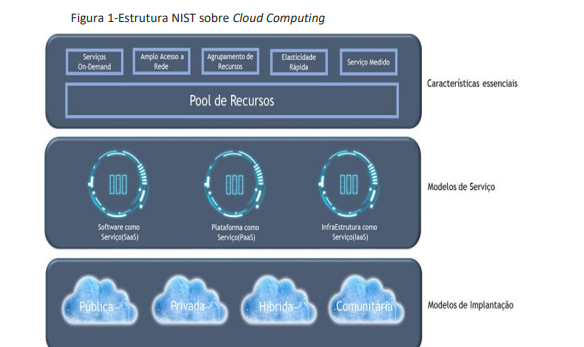
\includegraphics[height=5cm]{pic/imagem_2024-09-20_150349691.png}
		\caption{Fonte: Adaptado de NIST SP 800-145, “A NIST definition of cloud
computing”,http://csrc.nist.gov/publications/drafts/800-145/Draft-SP-800-
145_cloud-definition.pdf}
		\label{fig:unilogo}
	\end{figure}
\end{frame}


% Results --- --- --- --- --- --- --- --- --- --- --- 
\section{Conclusão}
\begin{frame}
    \begin{itemize}
        \item A computação em nuvem é essencial para o sucesso da Indústria 4.0.
        \item Ela oferece recursos escaláveis, facilita a automação e permite uma gestão de processos mais eficiente.
        \item Embora ainda em desenvolvimento, a nuvem já desempenha um papel crítico na modernização das indústrias, e sua importância só tende a crescer com o avanço da digitalização e novas tecnologias emergentes.

    \end{itemize}
\end{frame}


% --- Thank you slide ---
\begin{frame}
\begin{center}
{ Obrigado pela atenção}
\vspace{1cm}

Arthur Xavier e  Guilherme Vieira \\[1em]

\end{center}
\end{frame}

\end{document}